\chapter{Caso di Studio: Il Computer di Bordo dell'F-16}
\label{ch:f16_computer}
\label{sec:caso_di_studio}
\label{caso_di_studio_FCS}
Il caso di studio analizzato dal progetto tratta la simulazione del computer di bordo di un caccia F-16, l'implementazione in \texttt{src/app/F16\_Computer/F16\_Computer.cpp}. Questo programma istanzia simultaneamente su 7 core fisici, ciascuno dei quali è un sottosistema avionico distinto del velivolo, infatti ogni sotto-sistema esegue la propria Periodic Task attraverso la politica di schedulazione \textit{Rate Monotonic}.
L'obiettivo è duplice: dimostrare che l'architettura delle librerie sviluppate (si veda il Capitolo \ref{ch:librerie_core}) riesce a gestire correttamente scenari ad alto parallelismo e a validare che il sistema di tracciamento e analisi sia in grado di gestire e rappresentare graficamente thread concorrenti, producendo metriche temporali coerenti per ogni sottosistema creato.
 
% ============================================================================
\clearpage
\section{Motivazione Aeronautica e Architettura del Sistema}
% ============================================================================
Un computer di bordo avionico reale gestisce in parallelo subsistemi con requisiti temporali diversi la creazione che seguirà avrà come bibliografia di base la seguente 	\cite{Scheduling_Real_Time}, ad esempio i loop di controllo del volo devono reagire in pochi millisecondi, mentre i radar e i display possono tollerare periodi più lunghi. Questo permette di testare se la schedulazione \textit{Rate Monotonic}, o nel caso si utilizzi un qualsiasi altro algoritmo di schedulazione, ad ogni task viene permesso di eseguire la propria Periodic Task senza superare la deadline, garantendo che i task più critici ottengano sempre la CPU per eseguire in modo che non si presentino deadline miss che facciano degradare la risposta del sistema.
Il simulatore F-16 è stato strutturato in sei \texttt{sub-systems} rispecchiando l'architettura aviconica reale del velivolo preso in esame:

\begin{table}[htbp]
	\centering
	\caption{Mappa completa dei 20 thread del simulatore F-16}
	\label{tab:f16_threads}
	\begin{tabular}{|l|l|c|c|c|}
		\hline
		\textbf{Sottosistema} & \textbf{Thread} & \textbf{Core} & \textbf{Periodo (ms)} & \textbf{Priorità} \\
		\hline
		\multirow{3}{*}{FCS Longitudinal} & PITCH\_A & 0 & 10 & 98 \\
		& PITCH\_B & 1 & 10 & 98 \\
		& PITCH\_C & 2 & 10 & 98 \\
		\hline
		\multirow{3}{*}{FCS Lateral} & ROLL\_A & 3 & 10 & 98 \\
		& ROLL\_B & 4 & 10 & 98 \\
		& ROLL\_C & 5 & 10 & 98 \\
		\hline
		\multirow{2}{*}{FCS Altitude} & ALT\_A & 6 & 20 & 97 \\
		& ALT\_B & 0 & 20 & 97 \\
		\hline
		\multirow{2}{*}{Navigation GPS} & GPS\_1 & 1 & 50 & 94 \\
		& GPS\_2 & 2 & 50 & 94 \\
		\hline
		\multirow{3}{*}{Navigation INS} & INS\_1 & 3 & 10 & 98 \\
		& INS\_2 & 4 & 10 & 98 \\
		& INS\_3 & 5 & 10 & 98 \\
		\hline
		Radar Aereo & RADAR\_A & 6 & 50 & 94 \\
		\hline
		Radar Terrestre & RADAR\_G & 0 & 100 & 89 \\
		\hline
		\multirow{2}{*}{Engine FADEC} & FADEC\_A & 1 & 10 & 98 \\
		& FADEC\_B & 2 & 10 & 98 \\
		\hline
		Weapons & WEAPONS & 3 & 100 & 89 \\
		\hline
		\multirow{2}{*}{Displays} & HUD & 4 & 30 & 96 \\
		& MFD & 5 & 30 & 96 \\
		\hline
	\end{tabular}
\end{table}

% ============================================================================
\clearpage
\section{Librerie Avioniche Utilizzate}
% ============================================================================
Il simulatore non utilizza la libreria \texttt{activity} generica (descritta nella Sezione \ref{sec:lib_activity}), ma impiega le librerie  specifiche create appositamente per il modello F-16 illustrate nella Sezione \ref{sec:lib_f16}. Ogni sottosistema  corrisponde quindi a una libreria statica dedicata:

\begin{lstlisting}[language=C++, caption={Include delle librerie avioniche in F16\_Computer.cpp}]
	#include "f16_fcs_long.hpp"    // FCS Longitudinale (Beccheggio)
	#include "f16_fcs_lat.hpp"     // FCS Laterale (Rollio)
	#include "f16_fcs_alt.hpp"     // FCS Quota (Altitudine)
	#include "f16_nav_gps.hpp"     // Navigazione GPS
	#include "f16_nav_ins.hpp"     // Navigazione Inerziale
	#include "f16_radar_air.hpp"   // Radar aria-aria
	#include "f16_radar_gnd.hpp"   // Radar aria-terra
	#include "f16_engine_fadec.hpp"// Controllo Motore FADEC
	#include "f16_weapons.hpp"     // Sistema d'Arma
	#include "f16_displays.hpp"    // Display Avionici (HUD/MFD)
	#include "trace_marker.h"      // Marker di tracciamento kernel
\end{lstlisting}

\subsection{Modulo F-16: Librerie di Simulazione Aerodinamica}
\label{sec:lib_f16}

I moduli F-16 estendono il pattern della libreria \texttt{activity} con due funzionalità aggiuntive:

\subsubsection{Rilevamento Runtime delle Deadline Miss e Flag Skip}

\begin{lstlisting}[language=C++, caption={Logica di rilevamento deadline miss e skip nei moduli F-16}]
	exec_end_time = time_current_millisecs();
	
	if (exec_end_time > exec_next_release_time) {
		// La funzione ha usato piu' tempo del periodo disponibile:
		// segnala la violazione e attiva il flag di skip
		printf("%s:   -MISS-   cost = %ld ms\n",
		activity.name, computational_cost);
		skip = true;
	} else {
		printf("%s:   DO JOB   cost = %ld ms\n",
		activity.name, computational_cost);
	}
	
	// Al ciclo successivo, se skip e' true:
	if (skip) {
		printf("%s:   *SKIP*\n", activity.name);
		skip = false;
		// Salta l'esecuzione e va direttamente al clock_nanosleep
		goto wait_next_release;
	}
\end{lstlisting}

\paragraph{Perché skippare il ciclo successivo.}
Quando un task supera il proprio periodo, al ciclo successivo il tempo di rilascio calcolato (\texttt{exec\_next\_release\_time}) è già nel passato. Se il task eseguisse normalmente, uscirebbe immediatamente dal \texttt{clock\_nanosleep} senza effettivamente dormire poiché l'istante target è già trascorso quindi di conseguenza inizierebbe subito un nuovo ciclo di esecuzione. Il risultato sarebbe che il task esegue \textbf{due cicli consecutivi senza pausa}, consumando quasi il doppio della propria quantità di CPU e causando in questo modo certamente una seconda deadline miss che va a degradare le capacità del sistema. Il flag \texttt{skip} interrompe questo effetto a catena: al ciclo immediatamente successivo alla miss, il task non esegue la propria funzione applicativa ma va direttamente al \texttt{clock\_nanosleep}, lasciando il tempo al sistema di riallinearsi. Il costo di questo meccanismo è un ciclo ``vuoto'' in cui nessun dato viene elaborato, ma è il prezzo necessario per evitare un'instabilità a cascata.

\subsubsection{Elenco Completo dei Moduli F-16}

Ciascuno dei seguenti moduli basato sulla creazione di un \textbf{FCS} (flight control system), compila un archivio statico dedicato in \texttt{bin/lib/}. Il parametro \texttt{parameter} presente ogni modulo è stato creato  per produrre un carico computazionale, che durante l'esecuzione della simulazione,che assicuri la fine del periodic task entro la deadline di riferimento:

\begin{itemize}
	\item \textbf{\texttt{engine\_fadec}} $\rightarrow$ \texttt{libf16\_engine\_fadec.a}: simula il controllo digitale del motore tramite calcoli del flusso di carburante (\texttt{exp(sin(i)) * cos(i)}). Ha il meccanismo di skip attivo perché il controllo motore è safety-critical: una miss non può essere ignorata senza conseguenze.
	\item \textbf{\texttt{fcs\_long}} $\rightarrow$ \texttt{libf16\_fcs\_long.a}: sistema di controllo longitudinale (beccheggio). Periodo nominale 10 ms.
	\item \textbf{\texttt{fcs\_lat}} $\rightarrow$ \texttt{libf16\_fcs\_lat.a}: sistema di controllo laterale (rollio). Periodo nominale 10 ms.
	\item \textbf{\texttt{fcs\_alt}} $\rightarrow$ \texttt{libf16\_fcs\_alt.a}: controllo automatico della quota. Periodo nominale 20 ms.
	\item \textbf{\texttt{nav\_gps}} $\rightarrow$ \texttt{libf16\_nav\_gps.a}: simulazione ricezione e filtraggio segnali GPS. Periodo nominale 50 ms.
	\item \textbf{\texttt{nav\_ins}} $\rightarrow$ \texttt{libf16\_nav\_ins.a}: navigazione inerziale con integrazione degli accelerometri. Periodo nominale 10 ms (stessa frequenza del FCS).
	\item \textbf{\texttt{radar\_air}} $\rightarrow$ \texttt{libf16\_radar\_air.a}: elaborazione segnali radar aria-aria. Periodo nominale 50 ms, carico più elevato (\texttt{parameter = 10}).
	\item \textbf{\texttt{radar\_gnd}} $\rightarrow$ \texttt{libf16\_radar\_gnd.a}: radar di mappatura terrestre. Periodo nominale 100 ms, carico massimo (\texttt{parameter = 15}).
	\item \textbf{\texttt{weapons}} $\rightarrow$ \texttt{libf16\_weapons.a}: logica del sistema d'arma. Periodo nominale 100 ms.
	\item \textbf{\texttt{displays}} $\rightarrow$ \texttt{libf16\_displays.a}: aggiornamento display avionici HUD e MFD. Periodo nominale 30 ms.
\end{itemize}

Ogni libreria espone la propria struttura di parametrizzazione (es. \texttt{t\_f16\_fcs\_long\_par}) e la propria funzione \texttt{PeriodicTask\_<NOME>} che internamente utilizza le primitive della libreria \texttt{time} (Sezione \ref{sec:lib_time}) per il sincronismo assoluto e la libreria \texttt{trace} (Sezione \ref{sec:lib_trace}) per la marcatura del kernel.

% ============================================================================
\section{Il Sistema di Controllo del Volo (FCS)}
% ============================================================================
Il Flight Control System \cite{nasa1984}, è il sottosistema più importante ed infatti è proprio questo sistema che garantisce la sicurezza durante il volo in condizione di volo anche da combattimento. I controlli più importanti sono i loop di controllo per beccheggio (\textit{pitch}), rollio (\textit{roll}) e quota (\textit{altitude}) quest'ultimi devono rispettare deadline strettissime affinché il velivolo rimanga stabile.

\subsection{Controllo del Beccheggio (PITCH\_A, PITCH\_B, PITCH\_C)}
I tre thread \texttt{PITCH\_A}, \texttt{PITCH\_B} e \texttt{PITCH\_C} implementano un controllo longitudinale: operano in parallelo su tre core distinti (Core 0, 1 e 2) con lo stesso periodo di \textbf{10 ms}. La presenza di tre thread è una caratteristica di sicurezza.

\begin{lstlisting}[language=C++, caption={Creazione del thread PITCH\_A su Core 0 con periodo 10 ms}]
	// Affinita': Core 0 dedicato esclusivamente a PITCH_A
	CPU_ZERO(&cpuset); CPU_SET(0, &cpuset);
	pthread_attr_setaffinity_np(&attr_pitch_a, sizeof(cpu_set_t), &cpuset);
	
	t_f16_fcs_long_par activity_pitch_a;
	sprintf(activity_pitch_a.name, "PITCH_A");
	activity_pitch_a.period    = 10;   // ms  deadline critica
	activity_pitch_a.parameter = 2;    // carico computazionale ridotto
	activity_pitch_a.deadline  = 10;   // ms  coincidente con il periodo
	
	// Priorita Rate Monotonic: 99 - (10/10) = 98 (altissima)
	param_pitch_a.sched_priority = 99 - (activity_pitch_a.period / 10);
	pthread_attr_setschedparam(&attr_pitch_a, &param_pitch_a);
	
	ret_err = pthread_create(&thread_pitch_a, &attr_pitch_a,
	PeriodicTask_FCS_LONG, (void *)&activity_pitch_a);
	pthread_setname_np(thread_pitch_a, "PITCH_A");
\end{lstlisting}

La scelta del parametro \texttt{2} (carico computazionale) è calibrata per garantire che l'esecuzione della funzione aviconica sia completata entro i 10 ms di deadline. Analogamente vengono creati \texttt{PITCH\_B} (Core 1) e \texttt{PITCH\_C} (Core 2).

\subsection{Controllo del Rollio (ROLL\_A, ROLL\_B, ROLL\_C)}
Il controllo laterale segue la stessa logica. I tre thread \texttt{ROLL\_A}, \texttt{ROLL\_B}, \texttt{ROLL\_C} vengono assegnati ai Core 3, 4 e 5 con periodo \textbf{10 ms}, garantendo che il controllo degli alettoni sia completamente isolato dal controllo del beccheggio a livello hardware.

\subsection{Controllo della Quota (ALT\_A, ALT\_B)}
I thread \texttt{ALT\_A} e \texttt{ALT\_B} gestiscono il mantenimento automatico della quota. Con periodo \textbf{20 ms} (il doppio dei loop di controllo primari), ottengono una priorità leggermente inferiore (97 vs 98), rispettando la gerarchia \textit{Rate Monotonic}: il controllo degli assetti primari deve sempre precedere il controllo della quota in caso di contesa.

\begin{lstlisting}[language=C++, caption={Configurazione di ALT\_A: periodo 20 ms, priorità 97}]
	t_f16_fcs_alt_par activity_alt_a;
	sprintf(activity_alt_a.name, "ALT_A");
	activity_alt_a.period    = 20;
	activity_alt_a.parameter = 3;
	activity_alt_a.deadline  = 20;
	
	// Priorita RM: 99 - (20/10) = 97
	param_alt_a.sched_priority = 99 - (activity_alt_a.period / 10);
\end{lstlisting}

% ============================================================================

\section{Il Sistema di Navigazione}
% ============================================================================
Il sistema di navigazione implementato in real-time si basa sull'architettura descritta in \cite{Navigation_System}. In tale contesto viene simulata l'azione di due tecnologie complementari: la ricezione GPS per la posizione assoluta e la navigazione inerziale per la stima continua dello stato cinematico del velivolo.

\subsection{Navigazione GPS (GPS\_1, GPS\_2)}
I due thread GPS operano a \textbf{50 ms} (20 Hz), frequenza compatibile con la banda tipica dei ricevitori GPS ad alta precisione. Vengono assegnati ai Core 1 e 2.

\subsection{Navigazione Inerziale (INS\_1, INS\_2, INS\_3)}
Il sistema inerziale è il più critico nell'architettura di navigazione: con periodo \textbf{10 ms} gestito su i tre (Core 3, 4 e 5), i tre thread INS ottengono priorità 98, identica ai loop FCS. La navigazione inerziale deve essere aggiornata alla stessa frequenza dei controlli di volo perché fornisce i dati di assetto in tempo reale utilizzati dal FCS:

\begin{lstlisting}[language=C++, caption={Configurazione del sistema INS}]
	// INS_1 su Core 3
	t_f16_nav_ins_par activity_ins_1;
	sprintf(activity_ins_1.name, "INS_1");
	activity_ins_1.period    = 10;    // ms  stessa frequenza del FCS
	activity_ins_1.parameter = 4;     // carico maggiore del GPS (elaborazione IMU)
	activity_ins_1.deadline  = 10;
	
	// INS_2 su Core 4, INS_3 su Core 5  stessi parametri
\end{lstlisting}

% ============================================================================
\clearpage
\section{Il Sistema Radar}
% ============================================================================
Il computer di bordo creato implementa due modalità radar con requisiti temporali differenziati, riflettendo le caratteristiche operative reali del radar AN/APG-68 \cite{Radar_AN/APG-68}, montato sull'F-16.

\subsection{Radar Aria-Aria (RADAR\_A)}
Il thread \texttt{RADAR\_A} opera con periodo \textbf{50 ms} sul Core 6. Con parametro \texttt{10}, genera il carico computazionale più elevato dell'intera architettura, simulando l'elaborazione dei segnali radio-frequenza per il tracciamento di bersagli aerei.

\subsection{Radar Aria-Terra (RADAR\_G)}
Il radar di mappatura terrestre \texttt{RADAR\_G} opera con periodo \textbf{100 ms} sul Core 0, ottenendo la priorità più bassa tra i radar (89). L'aggiornamento meno frequente riflette la minore urgenza della mappatura del suolo rispetto al tracciamento di minacce aeree:

\begin{lstlisting}[language=C++, caption={Configurazione di RADAR\_G: periodo 100 ms, massimo carico}]
	t_f16_radar_gnd_par activity_radar_g;
	sprintf(activity_radar_g.name, "RADAR_G");
	activity_radar_g.period    = 100;  // ms aggiornamento meno critico
	activity_radar_g.parameter = 15;   // massimo carico computazionale
	activity_radar_g.deadline  = 100;
	
	// Priorita RM: 99 - (100/10) = 89
	param_radar_g.sched_priority = 99 - (activity_radar_g.period / 10);
\end{lstlisting}

% ============================================================================
\clearpage
\section{Il Sistema FADEC}
% ============================================================================
Il FADEC (\textit{Full Authority Digital Engine Control})\cite{spitzer2017digital}, è il sistema che gestisce in modo digitale il controllo completo del motore turbofan General Electric F110 dell'F-16. I due thread \texttt{FADEC\_A} e \texttt{FADEC\_B} operano con periodo \textbf{10 ms} sui Core 1 e 2, con priorità 98, affiancando i loop di controllo del volo nella fascia temporale più critica.

Il parametro computazionale \texttt{3} genera all'interno della libreria \texttt{f16\_engine\_fadec} (Sezione \ref{sec:lib_f16}) una simulazione del calcolo del flusso di carburante tramite la funzione \texttt{exp(sin(i)) * cos(i)}, ed è dotato del meccanismo di rilevamento delle deadline miss con flag \texttt{skip} descritto nel capitolo delle librerie:

\begin{lstlisting}[language=C++, caption={Configurazione del thread FADEC\_A}]
	t_f16_engine_fadec_par activity_fadec_a;
	sprintf(activity_fadec_a.name, "FADEC_A");
	activity_fadec_a.period    = 10;   // ms  controllo motore critico
	activity_fadec_a.parameter = 3;
	activity_fadec_a.deadline  = 10;
	
	// Priorita 98: identica ai loop FCS e INS
	param_fadec_a.sched_priority = 99 - (activity_fadec_a.period / 10);
	ret_err = pthread_create(&thread_fadec_a, &attr_fadec_a,
	PeriodicTask_ENGINE_FADEC, (void *)&activity_fadec_a);
	pthread_setname_np(thread_fadec_a, "FADEC_A");
\end{lstlisting}

% ============================================================================
\section{Il Sistema d'Arma e i Display Avionici}
% ============================================================================

\subsection{Sistema d'ingaggio}
Il thread \texttt{WEAPONS} gestisce la logica del sistema missilistico e del cannone M61A1. Con periodo \textbf{100 ms} sul Core 3, ottiene la priorità più bassa (89), riflettendo la natura non continua delle operazioni d'arma rispetto ai loop di controllo del volo 

\subsection{Display HUD e MFD}
I due thread di visualizzazione (\texttt{HUD} e \texttt{MFD}) operano a \textbf{30 ms} (circa 33 Hz) rispettivamente su Core 4 e Core 5. Il periodo di 30 ms garantisce una frequenza di aggiornamento fluida per il pilota mantenendo un margine adeguato rispetto ai loop critici da 10 ms.

% ============================================================================
\section{Distribuzione dei Core e Analisi dell'Architettura}
% ============================================================================
La distribuzione dei 20 thread sui 7 core fisici disponibili è il risultato di un bilanciamento architetturale che tiene conto sia della criticità temporale che del carico computazionale di ogni sottosistema. La Figura \ref{fig:f16_core_map} illustra la mappa di assegnazione.


Va notato che alcuni core ospitano thread di diversi sottosistemi con periodi differenti:
\begin{itemize}
	\item \textbf{Core 0:} ospita \texttt{PITCH\_A} (10 ms, priorità 98), \texttt{ALT\_B} (20 ms, priorità 97) e \texttt{RADAR\_G} (100 ms, priorità 89). Lo scheduler \texttt{SCHED\_FIFO} garantisce che \texttt{PITCH\_A} possa sempre prelazionare i task a priorità inferiore.
	\item \textbf{Core 1:} ospita \texttt{PITCH\_B} (10 ms), \texttt{GPS\_1} (50 ms) e \texttt{FADEC\_A} (10 ms). La coesistenza di due task con periodo 10 ms sullo stesso core è possibile solo se la loro esecuzione combinata non supera i 10 ms disponibili nel periodo.
\end{itemize}

% ============================================================================

\section{Sincronizzazione Finale e Terminazione}
% ============================================================================
Al termine della sezione di creazione dei thread, il \texttt{main} esegue una \texttt{pthread\_join} per ognuno dei 20 thread prima di chiudere il file descriptor dei marker:

\begin{lstlisting}[language=C++, caption={Attesa di terminazione di tutti i 20 thread}]
	pthread_join(thread_pitch_a, NULL);
	pthread_join(thread_pitch_b, NULL);
	pthread_join(thread_pitch_c, NULL);
	pthread_join(thread_roll_a, NULL);
	pthread_join(thread_roll_b, NULL);
	pthread_join(thread_roll_c, NULL);
	pthread_join(thread_alt_a, NULL);
	pthread_join(thread_alt_b, NULL);
	pthread_join(thread_gps_1, NULL);
	pthread_join(thread_gps_2, NULL);
	pthread_join(thread_ins_1, NULL);
	pthread_join(thread_ins_2, NULL);
	pthread_join(thread_ins_3, NULL);
	pthread_join(thread_radar_a, NULL);
	pthread_join(thread_radar_g, NULL);
	pthread_join(thread_fadec_a, NULL);
	pthread_join(thread_fadec_b, NULL);
	pthread_join(thread_weapons, NULL);
	pthread_join(thread_hud, NULL);
	pthread_join(thread_mfd, NULL);
	
	close_tracing();
	exit(0);
\end{lstlisting}

Poiché ogni thread esegue un loop infinito (\texttt{while(1)}), nella pratica il programma non termina spontaneamente: il \texttt{main} rimane bloccato sulle \texttt{pthread\_join} fino all'interruzione esterna da parte del sistema operativo (tipicamente tramite \texttt{Ctrl+C} o il termine dello script di tracciamento).
\clearpage
% ============================================================================

\section{Risultati dell'Analisi di Tracciamento}
% ============================================================================
Il tracciamento di \textbf{F16\_Computer} viene avviato tramite lo script \texttt{run\_trace.sh}:

\begin{lstlisting}[language=bash]
	cd bin/tools/
	./run_trace.sh F16_Computer
\end{lstlisting}

Al termine dell'acquisizione, il parser C++ \texttt{thread\_analysis} analizza il file \texttt{trace\_output.txt} riconoscendo tutti i 20 thread tramite i loro marker \texttt{PERIOD\_START\_<NOME>} e producendo il file \texttt{timeline.csv} con le statistiche complete.

\begin{figure}[htbp]
	\centering
	% Senza keepaspectratio, l'immagine viene forzata a queste esatte dimensioni
	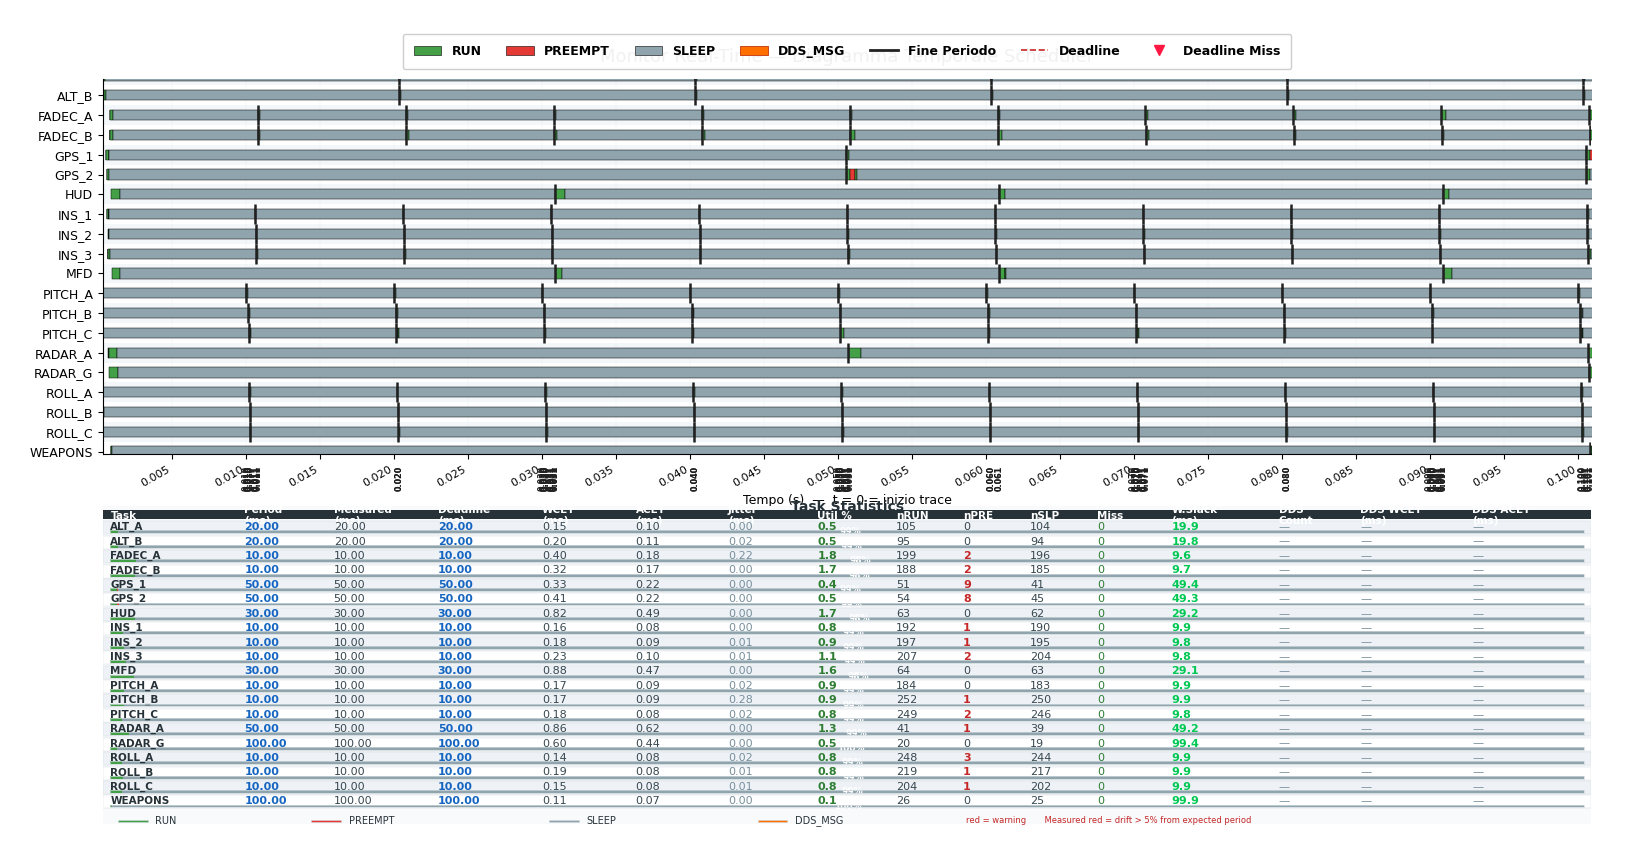
\includegraphics[width=1\textwidth, height=0.60\textheight]{Foto/Thread/F16Monitor.png}
	\caption{Diagramma di Gantt del simulatore F-16 prodotto da \texttt{monitor.py}: le 20 corsie temporali mostrano l'alternanza di stati \texttt{RUN} (verde), \texttt{SLEEP} (grigio) e \texttt{PREEMPT} (rosso) per ogni sottosistema avionico.}
	\label{fig:f16_gantt}
\end{figure}
\clearpage
\begin{lstlisting}[language=C++, caption={Attesa di terminazione di tutti i 20 thread}]
	----------------------------------------------------------
	TASK: PITCH_A (PID: 22440)
	----------------------------------------------------------
	[Esecuzione] WCET :      0.175 ms  |  ACET:      0.089 ms
	[T.Risposta] WCRT :      0.130 ms
	[Periodo]    Mis. :      9.999 ms  |  Jitter:    0.021 ms
	[Parametri]  Periodo:   10.000 ms  |  Deadline:   10.000 ms
	[Scadenze]   Miss   :        0      |  Slack Peggiore:    9.870 ms
	[Stati]      Sleep  :      183      |  Preempt:        0     |  Run n.: 184
	[Globale]    Util%  :    0.909 %    |  Gaps   :      183 (10.008 ms max)
	
	----------------------------------------------------------
	TASK: PITCH_B (PID: 22441)
	----------------------------------------------------------
	[Esecuzione] WCET :      0.170 ms  |  ACET:      0.088 ms
	[T.Risposta] WCRT :      0.126 ms
	[Periodo]    Mis. :     10.001 ms  |  Jitter:    0.278 ms
	[Parametri]  Periodo:   10.000 ms  |  Deadline:   10.000 ms
	[Scadenze]   Miss   :        0      |  Slack Peggiore:    9.874 ms
	[Stati]      Sleep  :      250      |  Preempt:        1     |  Run n.: 252
	[Globale]    Util%  :    0.891 %    |  Gaps   :      243 (12.530 ms max)
	
	----------------------------------------------------------
	TASK: PITCH_C (PID: 22442)
	----------------------------------------------------------
	[Esecuzione] WCET :      0.181 ms  |  ACET:      0.078 ms
	[T.Risposta] WCRT :      0.154 ms
	[Periodo]    Mis. :     10.000 ms  |  Jitter:    0.023 ms
	[Parametri]  Periodo:   10.000 ms  |  Deadline:   10.000 ms
	[Scadenze]   Miss   :        0      |  Slack Peggiore:    9.846 ms
	[Stati]      Sleep  :      246      |  Preempt:        2     |  Run n.: 249
	[Globale]    Util%  :    0.799 %    |  Gaps   :      236 (9.991 ms max)
	
	----------------------------------------------------------
	TASK: ROLL_A (PID: 22443)
	----------------------------------------------------------
	[Esecuzione] WCET :      0.139 ms  |  ACET:      0.076 ms
	[T.Risposta] WCRT :      0.120 ms
	[Periodo]    Mis. :     10.001 ms  |  Jitter:    0.022 ms
	[Parametri]  Periodo:   10.000 ms  |  Deadline:   10.000 ms
	[Scadenze]   Miss   :        0      |  Slack Peggiore:    9.880 ms
	[Stati]      Sleep  :      244      |  Preempt:        3     |  Run n.: 248
	[Globale]    Util%  :    0.778 %    |  Gaps   :      238 (10.028 ms max)
	
	----------------------------------------------------------
	TASK: ROLL_B (PID: 22444)
	----------------------------------------------------------
	[Esecuzione] WCET :      0.188 ms  |  ACET:      0.081 ms
	[T.Risposta] WCRT :      0.148 ms
	[Periodo]    Mis. :     10.000 ms  |  Jitter:    0.005 ms
	[Parametri]  Periodo:   10.000 ms  |  Deadline:   10.000 ms
	[Scadenze]   Miss   :        0      |  Slack Peggiore:    9.852 ms
	[Stati]      Sleep  :      217      |  Preempt:        1     |  Run n.: 219
	[Globale]    Util%  :    0.827 %    |  Gaps   :      214 (9.972 ms max)
	
	----------------------------------------------------------
	TASK: ROLL_C (PID: 22445)
	----------------------------------------------------------
	[Esecuzione] WCET :      0.149 ms  |  ACET:      0.078 ms
	[T.Risposta] WCRT :      0.126 ms
	[Periodo]    Mis. :     10.000 ms  |  Jitter:    0.006 ms
	[Parametri]  Periodo:   10.000 ms  |  Deadline:   10.000 ms
	[Scadenze]   Miss   :        0      |  Slack Peggiore:    9.874 ms
	[Stati]      Sleep  :      202      |  Preempt:        1     |  Run n.: 204
	[Globale]    Util%  :    0.790 %    |  Gaps   :      202 (9.975 ms max)
	
	----------------------------------------------------------
	TASK: ALT_A (PID: 22446)
	----------------------------------------------------------
	[Esecuzione] WCET :      0.149 ms  |  ACET:      0.100 ms
	[T.Risposta] WCRT :      0.132 ms
	[Periodo]    Mis. :     20.001 ms  |  Jitter:    0.002 ms
	[Parametri]  Periodo:   20.000 ms  |  Deadline:   20.000 ms
	[Scadenze]   Miss   :        0      |  Slack Peggiore:   19.868 ms
	[Stati]      Sleep  :      104      |  Preempt:        0     |  Run n.: 105
	[Globale]    Util%  :    0.509 %    |  Gaps   :      104 (19.921 ms max)
	
	----------------------------------------------------------
	TASK: ALT_B (PID: 22447)
	----------------------------------------------------------
	[Esecuzione] WCET :      0.201 ms  |  ACET:      0.105 ms
	[T.Risposta] WCRT :      0.182 ms
	[Periodo]    Mis. :     20.001 ms  |  Jitter:    0.021 ms
	[Parametri]  Periodo:   20.000 ms  |  Deadline:   20.000 ms
	[Scadenze]   Miss   :        0      |  Slack Peggiore:   19.818 ms
	[Stati]      Sleep  :       94      |  Preempt:        0     |  Run n.: 95
	[Globale]    Util%  :    0.537 %    |  Gaps   :       94 (20.034 ms max)
	
	----------------------------------------------------------
	TASK: GPS_1 (PID: 22448)
	----------------------------------------------------------
	[Esecuzione] WCET :      0.326 ms  |  ACET:      0.218 ms
	[T.Risposta] WCRT :      0.575 ms
	[Periodo]    Mis. :     50.002 ms  |  Jitter:    0.001 ms
	[Parametri]  Periodo:   50.000 ms  |  Deadline:   50.000 ms
	[Scadenze]   Miss   :        0      |  Slack Peggiore:   49.425 ms
	[Stati]      Sleep  :       41      |  Preempt:        9     |  Run n.: 51
	[Globale]    Util%  :    0.449 %    |  Gaps   :       49 (49.812 ms max)
	
	----------------------------------------------------------
	TASK: GPS_2 (PID: 22449)
	----------------------------------------------------------
	[Esecuzione] WCET :      0.407 ms  |  ACET:      0.224 ms
	[T.Risposta] WCRT :      0.696 ms
	[Periodo]    Mis. :     50.002 ms  |  Jitter:    0.002 ms
	[Parametri]  Periodo:   50.000 ms  |  Deadline:   50.000 ms
	[Scadenze]   Miss   :        0      |  Slack Peggiore:   49.304 ms
	[Stati]      Sleep  :       45      |  Preempt:        8     |  Run n.: 54
	[Globale]    Util%  :    0.462 %    |  Gaps   :       50 (49.824 ms max)
	
	----------------------------------------------------------
	TASK: INS_1 (PID: 22450)
	----------------------------------------------------------
	[Esecuzione] WCET :      0.156 ms  |  ACET:      0.082 ms
	[T.Risposta] WCRT :      0.141 ms
	[Periodo]    Mis. :     10.000 ms  |  Jitter:    0.004 ms
	[Parametri]  Periodo:   10.000 ms  |  Deadline:   10.000 ms
	[Scadenze]   Miss   :        0      |  Slack Peggiore:    9.859 ms
	[Stati]      Sleep  :      190      |  Preempt:        1     |  Run n.: 192
	[Globale]    Util%  :    0.830 %    |  Gaps   :      188 (9.939 ms max)
	
	----------------------------------------------------------
	TASK: INS_2 (PID: 22451)
	----------------------------------------------------------
	[Esecuzione] WCET :      0.182 ms  |  ACET:      0.090 ms
	[T.Risposta] WCRT :      0.164 ms
	[Periodo]    Mis. :     10.000 ms  |  Jitter:    0.008 ms
	[Parametri]  Periodo:   10.000 ms  |  Deadline:   10.000 ms
	[Scadenze]   Miss   :        0      |  Slack Peggiore:    9.836 ms
	[Stati]      Sleep  :      195      |  Preempt:        1     |  Run n.: 197
	[Globale]    Util%  :    0.913 %    |  Gaps   :      195 (9.963 ms max)
	
	----------------------------------------------------------
	TASK: INS_3 (PID: 22452)
	----------------------------------------------------------
	[Esecuzione] WCET :      0.231 ms  |  ACET:      0.105 ms
	[T.Risposta] WCRT :      0.198 ms
	[Periodo]    Mis. :     10.000 ms  |  Jitter:    0.010 ms
	[Parametri]  Periodo:   10.000 ms  |  Deadline:   10.000 ms
	[Scadenze]   Miss   :        0      |  Slack Peggiore:    9.802 ms
	[Stati]      Sleep  :      204      |  Preempt:        2     |  Run n.: 207
	[Globale]    Util%  :    1.060 %    |  Gaps   :      204 (9.950 ms max)
	
	----------------------------------------------------------
	TASK: RADAR_A (PID: 22453)
	----------------------------------------------------------
	[Esecuzione] WCET :      0.859 ms  |  ACET:      0.621 ms
	[T.Risposta] WCRT :      0.849 ms
	[Periodo]    Mis. :     50.002 ms  |  Jitter:    0.003 ms
	[Parametri]  Periodo:   50.000 ms  |  Deadline:   50.000 ms
	[Scadenze]   Miss   :        0      |  Slack Peggiore:   49.151 ms
	[Stati]      Sleep  :       39      |  Preempt:        1     |  Run n.: 41
	[Globale]    Util%  :    1.278 %    |  Gaps   :       39 (49.448 ms max)
	
	----------------------------------------------------------
	TASK: RADAR_G (PID: 22454)
	----------------------------------------------------------
	[Esecuzione] WCET :      0.599 ms  |  ACET:      0.436 ms
	[T.Risposta] WCRT :      0.608 ms
	[Periodo]    Mis. :    100.004 ms  |  Jitter:    0.001 ms
	[Parametri]  Periodo:  100.000 ms  |  Deadline:  100.000 ms
	[Scadenze]   Miss   :        0      |  Slack Peggiore:   99.392 ms
	[Stati]      Sleep  :       19      |  Preempt:        0     |  Run n.: 20
	[Globale]    Util%  :    0.472 %    |  Gaps   :       19 (99.667 ms max)
	
	----------------------------------------------------------
	TASK: FADEC_A (PID: 22455)
	----------------------------------------------------------
	[Esecuzione] WCET :      0.404 ms  |  ACET:      0.175 ms
	[T.Risposta] WCRT :      0.383 ms
	[Periodo]    Mis. :     10.000 ms  |  Jitter:    0.218 ms
	[Parametri]  Periodo:   10.000 ms  |  Deadline:   10.000 ms
	[Scadenze]   Miss   :        0      |  Slack Peggiore:    9.617 ms
	[Stati]      Sleep  :      196      |  Preempt:        2     |  Run n.: 199
	[Globale]    Util%  :    1.765 %    |  Gaps   :      198 (11.945 ms max)
	
	----------------------------------------------------------
	TASK: FADEC_B (PID: 22456)
	----------------------------------------------------------
	[Esecuzione] WCET :      0.319 ms  |  ACET:      0.167 ms
	[T.Risposta] WCRT :      0.300 ms
	[Periodo]    Mis. :     10.000 ms  |  Jitter:    0.005 ms
	[Parametri]  Periodo:   10.000 ms  |  Deadline:   10.000 ms
	[Scadenze]   Miss   :        0      |  Slack Peggiore:    9.700 ms
	[Stati]      Sleep  :      185      |  Preempt:        2     |  Run n.: 188
	[Globale]    Util%  :    1.680 %    |  Gaps   :      187 (9.884 ms max)
	
	----------------------------------------------------------
	TASK: WEAPONS (PID: 22457)
	----------------------------------------------------------
	[Esecuzione] WCET :      0.114 ms  |  ACET:      0.074 ms
	[T.Risposta] WCRT :      0.092 ms
	[Periodo]    Mis. :    100.004 ms  |  Jitter:    0.002 ms
	[Parametri]  Periodo:  100.000 ms  |  Deadline:  100.000 ms
	[Scadenze]   Miss   :        0      |  Slack Peggiore:   99.908 ms
	[Stati]      Sleep  :       25      |  Preempt:        0     |  Run n.: 26
	[Globale]    Util%  :    0.079 %    |  Gaps   :       24 (99.948 ms max)
	
	----------------------------------------------------------
	TASK: HUD (PID: 22458)
	----------------------------------------------------------
	[Esecuzione] WCET :      0.824 ms  |  ACET:      0.494 ms
	[T.Risposta] WCRT :      0.806 ms
	[Periodo]    Mis. :     30.001 ms  |  Jitter:    0.002 ms
	[Parametri]  Periodo:   30.000 ms  |  Deadline:   30.000 ms
	[Scadenze]   Miss   :        0      |  Slack Peggiore:   29.194 ms
	[Stati]      Sleep  :       62      |  Preempt:        0     |  Run n.: 63
	[Globale]    Util%  :    1.685 %    |  Gaps   :       62 (29.642 ms max)
	----------------------------------------------------------
	TASK: MFD (PID: 22459)
	----------------------------------------------------------
	[Esecuzione] WCET :      0.880 ms  |  ACET:      0.469 ms
	[T.Risposta] WCRT :      0.865 ms
	[Periodo]    Mis. :     30.001 ms  |  Jitter:    0.002 ms
	[Parametri]  Periodo:   30.000 ms  |  Deadline:   30.000 ms
	[Scadenze]   Miss   :        0      |  Slack Peggiore:   29.135 ms
	[Stati]      Sleep  :       63      |  Preempt:        0     |  Run n.: 64
	[Globale]    Util%  :    1.590 %    |  Gaps   :       62 (29.630 ms max)
\end{lstlisting}
